\documentclass{article}
\usepackage[utf8]{inputenc}
\usepackage{emnlp16}
\usepackage{graphicx,hyperref}
\usepackage{tabularx}
\usepackage[table,xcdraw]{xcolor}

\newcommand{\ms}[1]{{\color{cyan}\{\textit{#1}\}$_{ms}$}}
\newcommand{\lhl}[1]{{\color{magenta}\{\textit{#1}\}$_{lhl}$}}

\title{Benchmarking Python Deep Learning Frameworks\\ for Language Modeling on GPUs}
% feel free to make this title much much better!
\emnlpfinalcopy 

\author{Lucy Lin, George Mulcaire \& Maarten Sap
\\University of Washington}
\date{December 2016}

\begin{document}

\maketitle

\begin{abstract}
Neural networks are omnipresent in natural language processing. 
We benchmark three popular Python frameworks (DyNet, TensorFlow and Theano) on a realistic NLP task: language modeling.
\ms{Change if needed:} We find that DyNet is significantly faster on this task. However, performance wasn't the only bottleneck during development, and there are other variables to consider.
\end{abstract}


\section{Introduction}
In recent years, deep learning approaches have exploded in popularity due to their performance gains over traditional systems on many tasks. Several deep learning frameworks have been released in response to this, each claiming niche improvements over others, but it is not necessarily clear which frameworks are better suited for which types of applications. Previous comparisons may now be out-of-date (older versions; lack of newer frameworks) or were run against simpler tasks (which might have hidden other interesting performance characteristics).

In this project, we benchmark deep learning frameworks on a complex natural language processing task and rank them based on different performance metrics. Specifically, we look at the following frameworks:
\begin{itemize}
	\item TensorFlow \cite{tensorflow}
	\item Theano \cite{theano}, using the Keras wrapper \cite{keras}
	\item DyNet \cite{dynet}
\end{itemize}
In natural language processing (NLP), recurrent neural networks (RNNs) are of particular interest because they make use of the sequential nature of language. Benchmarks on RNNs have been run before, but most tasks were benchmarked on toy tasks which do not necessarily reflect performance on real data. For instance, GitHub user \verb!glample! generated random data to run through their RNN \cite{glample}, which is not realistic. In NLP, we usually turn words into vocabulary-sized one-hot vectors and then embed them (i.e. dimensionality reduction) as hidden-sized vectors. Sparsely learning the embedding matrix, which is usually in the order of $[20,000 \times 200]$, is likely to severely impact performance.

\section{Background}
\subsection{Language Modeling}
The task of language modeling is about estimating probabilities of particular sequences of words. It is used as an invaluable component in various real-world applications such as speech recognition, statistical machine translation, etc. More formally, if $s=\{START,x_1,x_2,...,x_n,STOP\}$ is an n-word sentence, language modelling will try to estimate, for each word $x_i$
its probability given its history: $p(x_i|START,x_1,x_2,...,x_{i-1})$. 
Historically, this task can be done rather simply using an l-th order Markov model, where $p(x_i|START,x_1,x_2,...,x_{i-1}) = p(x_i|x_{i-l},x_{i-l+1},...,x_{i-1})$. However, the Markov assumption does not need to be made with recurrent neural networks, as they have the capabilities to encode much longer histories. With RNNs, we normalize (using softmax) the output of a nonlinear function $f\left(p(x_i|START,x_1,x_2,...,x_{i-1})\right) =softmax\left(f(x_i,START,x_1,x_2,...,x_{i-1})\right)$.

\subsection{Frameworks}
All three frameworks use a symbolic computation graph, which maps operations and variables to nodes in a graph. To perform a computation, one has to ``query'' the graph by providing values for variables needed to compute the desired output.
Figure~\ref{fig:compGraph} shows an example of a simple computation graph.

\begin{figure}\begin{center}
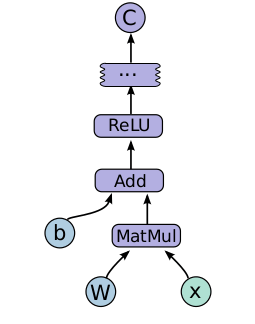
\includegraphics[scale=.4]{graphics/tensorflowGraph.png}
\caption{\label{fig:compGraph}Simple neural computation graph example. (\texttt{ReLU} is a rectified linear unit.) Figure is taken from \protect\cite{tensorflow}.} 
\end{center}\end{figure}

The frameworks handle computation graphs differently. Theano and Tensorflow perform ``static'' declaration of computation graphs: first, the graph architecture is specified, and then data is run through the compiled graph to train or make predictions. In contrast, DyNet does ``dynamic'' declaration of computation graphs; that is, the computation graph is defined on-the-fly as operations are executed.

All of the frameworks we tested have Python APIs\footnote{DyNet was originally a C++ framework which now has a Python wrapper; currently its Python wrapper only supports Python 2. TensorFlow and Theano are primarily Python frameworks that support both Python 2 and 3.} that wrap C++ or optimized Python code (e.g., numpy).

For speed, the frameworks all use fast low-level linear algebra libraries for matrix and tensor operations. Both TensorFlow and DyNet make extensive use of the Eigen library for C++, while Theano uses BLAS instead.


%TensorFlow's computation graph is pure \texttt{Python}, which makes it slower than other frameworks.

\section{Experiments}
\subsection{Data \& Preprocessing}
We chose to focus on the Los Angeles Times subset from 2009 of the GigaWord corpus \cite{gigaword}. Each of these documents is a news article, so we used NLTK’s \cite{nltk} sentence splitter on the articles. Every sentence is then tokenized using NLTK’s \verb!casual_tokenize! function, limiting ourselves to sentences that are $<100$ tokens long. In order to limit overfitting, we replace all words that occurred less than $150$ times by a special \verb!OOV! symbol (this allows the model to be more robust when encountering previously unseen words). We ended up with $1,191,848$ sentences, $27,269,856$ total word tokens and a vocabulary size of $35,642$.

\subsection{Implementation \& Hyperparameters}
\ms{Add equations/words to explain what a neural LM does.}
In our experiments, we optimized for a standard language modeling objective: \textit{cross-entropy}. The built-in cross-entropy loss functions in each framework were slightly different, which could potentially affect the number of iterations required for convergence. \ms{TODO: add github somewhere}

Table~\ref{tab:hyperparams} summarizes the hyperparameters chosen for the experiments; there was no cross-validation done since the evaluative performance of the model trained is irrelevant.
\begin{table}\begin{center}
\begin{tabular}{cc}
\textbf{hyperparam} & \textbf{value} \\\hline
RNN type & \texttt{LSTM} \\
hidden size & $256$ \\
optimizer & \texttt{AdamOptimizer} \\
learning rate & $0.003$ \\
batch size & 25 \\
\end{tabular}
\caption{\label{tab:hyperparams}Hyperparameters used in the experiments}
\end{center}\end{table}

Traditionally, neural models are trained until their performance on a \textit{development} set stops improving. Therefore, a full epoch of training (where all the training data is used) is usually followed by a predictive pass through development data.
\section{Benchmarks}
\subsection{Time}
The first benchmark to look at is how long training takes. Table \ref{tab:timing} summarizes various breakdowns. \ms{Summarize results: ie Dynet is the best (so far) (2 sentences perhaps)}.
\begin{table}
\begin{tabular}{c|ccc}
Time					& Dynet 		& TensorFlow 	& Theano \\ \hline
Convergence		& 26h10m 		& 35h25m 			& (TBD)\\
Train epoch 		& 2h20m		& 6h57m 			& 6h35m \\
Test epoch 		& 3m4s			& 7m45s 			& 24m \\
Train batch 		& 1s 				& 5s 					& 1s \\
Test batch 			& $<$1s 		& $<$1s 			& $<$1s \\
\end{tabular}
\caption{\label{tab:timing}Total runtime on various subtasks.}
\end{table}
\subsection{Function-level metrics}
Using NVidia's built-in GPU profiler, \verb!nvprof!, we measured various ways in which the different frameworks utilized the GPU hardware, specifically focusing on the matrix multiply operation implemented in the function \verb!magma_lds128_sgemm_kernel()!. Table \ref{tab:metrics} summarizes. \ms{Summarize results: i.e. they're all in the same order of magnitute, doesn't really tell us why DyNet would be much more efficient.
George TODO: explain the memset thing.}

\begin{table}
\centering
\begin{tabular}{c|rrr}
\textbf{Function} & Dynet &  TensorFlow & Theano \\  
\hline
matrix multiply & 29.64\%  &  68.87\% & 49.90\% \\
\hline
CUDA memset & 40.13\% & 0.00\% & 0.24\% \\
\end{tabular}

\caption{\label{tab:pcttime}Percentage of runtime spent on the most common matrix multiply call used (a variant of \texttt{\detokenize{magma_lds_128_sgemm_kernel()}}) and on CUDA memset operations. These numbers are from training on a single batch.}
\end{table}

\begin{table*}
\centering
\begin{tabular}{c|rrr}
\textbf{Metric} 										& \textbf{Dynet} & \textbf{TensorFlow} & \textbf{Theano} \\ \hline
\texttt{\detokenize{achieved_occupancy}}			&		0.062	&		0.062	&		0.062		\\
\texttt{\detokenize{sm_efficiency}}					&		16.64\%	&		22.58\%	&		16.04\%		\\
\texttt{\detokenize{warp_efficiency}}					&		100.0\%	&		100.0\%	&		99.99\%		\\
\texttt{\detokenize{warp_nonpred_efficiency}}	&		100.0\%	&		99.95\%	&		99.91\%		\\
\texttt{\detokenize{global_hit_rate}}					&		2.88\%	&		0.00\%	&		0.00\%		\\
\texttt{\detokenize{local_hit_rate}}					&		0.00\%	&		0.00\%	&		0.00\%		\\
\texttt{\detokenize{dram_read_throughput}} (GB/s)		&		10.07	&		11.07	 	&		9.97 	\\
\texttt{\detokenize{dram_write_throughput}} (MB/s)	&		357.63&		411.99 &		503.54	\\
\end{tabular}

\caption{\label{tab:metrics} Various CUDA profiler metrics for the task of training a single batch. Descriptions of these metrics are in section \ref{subsec:cudaprof}.}
\end{table*}


\subsection{Cuda Profiler}
\label{subsec:cudaprof}
We used the CUDA Profiler Toolkit \cite{nvprof} to characterize our implementations, specifically on a simplified task of training on one batch.

We profile which methods take the most amount of time, and look into a variety of metrics.
\begin{itemize}
\item \verb!achieved_occupancy! - number of GPU warps used vs. total number of warps available
\item \verb!sm_efficiency! - how much of the runtime is spent performing actual computation
\item \verb!warp_execution_efficiency! - how efficient is execution within a warp; number of registers per thread is likely a limiting factor for all implementations.
\item \verb!warp_nonpred_execution_efficiency! - how efficient is execution within a warp on non-predicated (i.e. non-branching) instructions.
\item \verb!dram_read_throughput! - read throughput from RAM to GPU
\item \verb!dram_write_throughput! - write throughput from GPU to RAM
\end{itemize}

\section{Discussion}
\ms{When looking to use neural network benchmarks, researchers might want to consider various aspects.}

\subsection{Performance}

\lhl{TODO: a higher-level summary of what we found in the benchmarks section.}
\ms{What do our results mean in term of selecting a framework, be broader in terms of how this is task specific.}

\subsection{Programmer Experience}

While implementing language models in these frameworks, we found that it is also important to consider the development experience. No one framework wins or loses out; instead, there are several tradeoffs to consider. We describe some of our experiences below.

\subsubsection{Installation/dependencies}

Unlike a standard Python module which just requires a simple \texttt{pip install}, neural network frameworks are typically dependent on external fast low-level linear algebra libraries to perform efficiently. Therefore there is often linking or configuration required to wire things together.

\lhl{TODO: fill in other installation bits}

\subsubsection{Ease of use}
\ms{TF pro: Google has money and resources.}
\lhl{TODO: all the things that TensorFlow/DyNet support out of the box.
comment somewhere about documentation, debuggability}

\paragraph{Theano} 
In contrast, Theano is ``lower-level'' in that it requires that the programmer define the shared variables, propagation steps, cost functions, and so on manually. Theano therefore offers a great deal of control and flexibility in model implementation, which is a benefit if one is implementing neural net layers not supported by other frameworks.

However, this also presents a steeper learning curve (despite the extensive documentation) and a much higher prototyping/development cost. We originally attempted to implement the Theano language model just using Theano and found the learning/debugging costs to be high. Because our language model consists of very standard neural net components, we instead switched to using Keras, which can use Theano under the covers but supplies an easier API with built-in RNN components.


\section{Conclusion}
\ms{Many factors, no clear winner; }

\section*{Acknowledgments}
We want to thank Emily Furst for helping us with GPU profiling, specifically understanding the CUDA Profiler documentation.
\newpage
\bibliography{references}
\bibliographystyle{emnlp16}
\end{document}
